\section{COVID-19 Datasets}

% Why do we need this dataset?

% What different sources did you look into and what are their pro's and con's. Are there alternatives?

% What did you do to prepare the dataset: cleaning, aligning, quality checking, balancing, etc.)

% include plots

% describe them

% Check if collected data is useful 

% Provide an assessment if you expect the data to be relevant for your project. In what way?
The main task in our research is to investigate the impact of the Covid-19 pandemic on greenhouse emissions, and its contribution to the countries, in achieving their goals of reducing emissions. So it was necessary to gather data on Covid-19 statistics of the countries, where it is available.
These statistics include, but are not limited to, the number of cases, deaths, recoveries, and ratios of these numbers to the population. We believe these numbers are responsible, together with each countries response to the pandemic, for the change in greenhouse emissions during the pandemic.
This data is vital to deduce the correlations between other data we have and predict the future of greenhouse emissions. In general, the datasets we have found and implemented are \begin{itemize}
	\item easy to access online or offline.
	\item updated frequently (at least daily).
	\item containing both Covid-19 data and coordinates of the corresponding region.
	\item containing data for both countries and smaller administrative regions.
	\item not containing general population data.
\end{itemize}

\subsection{Data Sources}
We have implemented ways of accessing data for two distinct datasets since it is best to compare different data sources for accuracy. Since external population data was needed for both datasets,
a dataset \cite{PopulationData} was downloaded and preprocessed to contain only the most recent population info, which is from 2018 except for Eritrea (2011).

\subsubsection{Bing}
The first dataset is provided by the Bing search engine \cite{Bing}. It is a CSV file, hosted on GitHub and updated every day by Microsoft. They collect data from multiple reliable sources, including WHO, state health departments, Wikipedia, etc.
Since it is hosted as a single file on GitHub, accessing the data in real-time is pretty straight-forward, by just providing the link to the file. The statistics in this dataset are the daily number of cases, deaths, recoveries. Moreover each there are samples for administrative regions within the countries and additional features are provided with each sample; last update date, coordinates, the country name in multiple ISO formats. The downside of this dataset is that it does not include any population data, so to calculate the ratios of
cases, deaths, and recoveries to the general population, the population for each country had to be accessed from a different dataset \cite{PopulationData}.

Firstly smaller administrative regions than countries were cleaned from the dataset since we are looking at the emission goals of countries and processing data for smaller administrative regions would be costly.
Then, to inspect the temporal change of the statistics for a selected country, the database can easily be filtered by the name of the country (since the samples are already sorted by date). But to inspect and create graphs on the most actual data,
all the samples but the most recent ones for each country were deleted. From there using the most actual data, all the features we have are drawn on world maps, with the help of Cartopy\cite{Cartopy}.


\begin{figure}[h]
	\centering
	\begin{subfigure}[b]{0.47\linewidth}
		\includegraphics[width=\linewidth]{covid/case rate}
	\end{subfigure}
	\begin{subfigure}[b]{0.47\linewidth}
		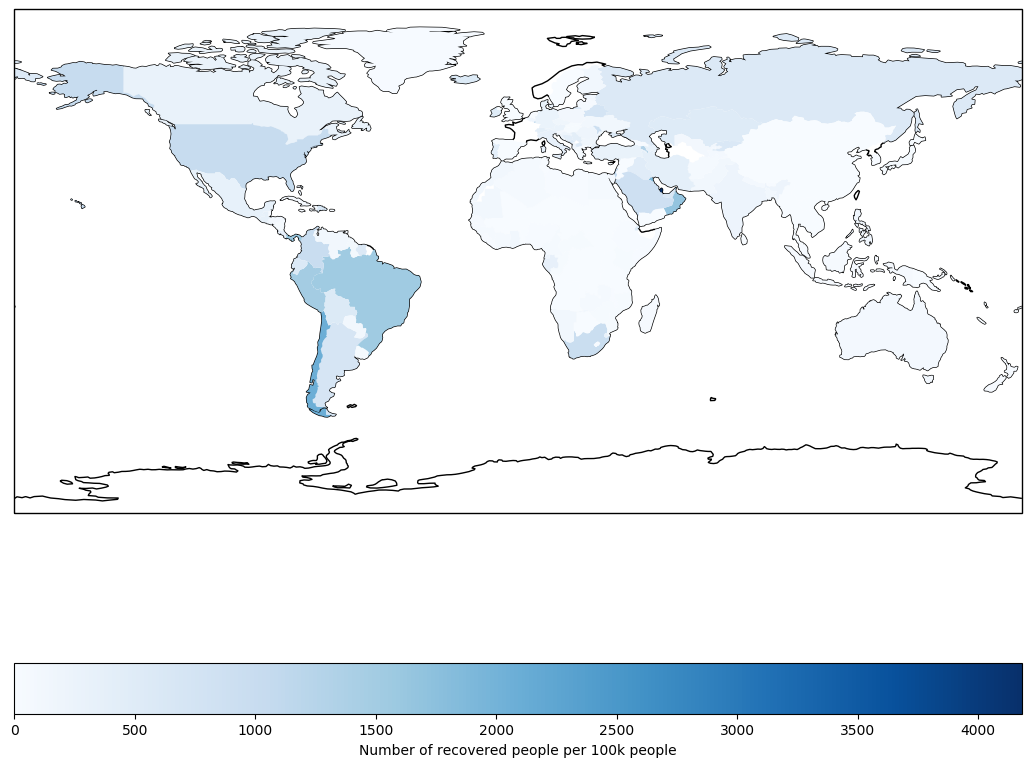
\includegraphics[width=\linewidth]{covid/recovered rate}
	\end{subfigure}
	\begin{subfigure}[b]{0.47\linewidth}
		\includegraphics[width=\linewidth]{covid/death rate}
	\end{subfigure}
	\caption{Covid-19 rates for each country.}
\end{figure}


\begin{figure}[h]
	\centering
	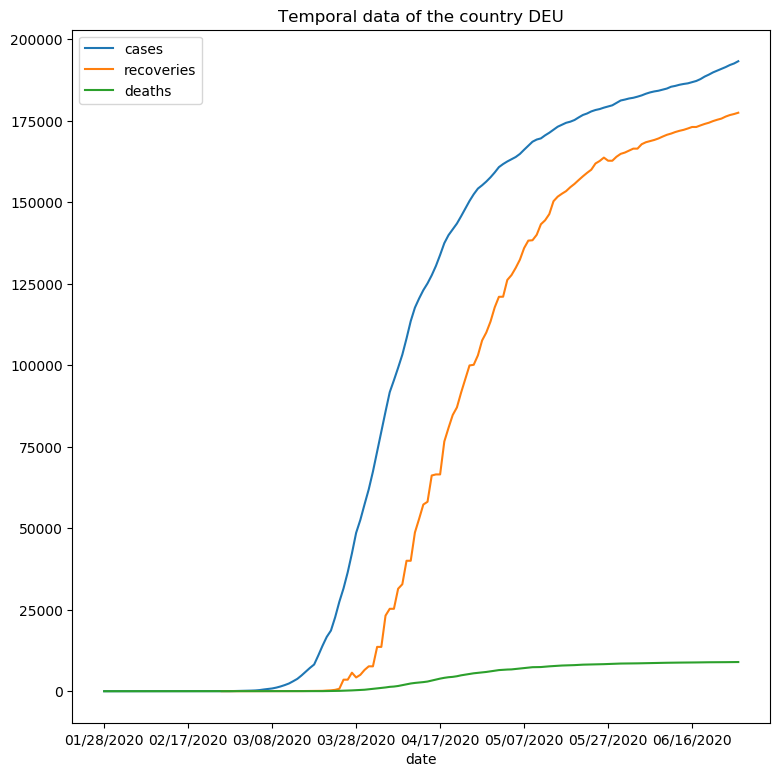
\includegraphics[width=0.50\linewidth]{covid/DEU}
	\caption{Temporal data of Germany. Drawn by using Bing dataset.}
\end{figure}

\subsubsection{Johns Hopkins CSSE}
The second dataset we use is provided by the Center for Systems Science and Engineering (CSSE) at Johns Hopkins University and gathered from multiple sources \cite{JohnsHopkins}.
In our project we access the dataset through https://covid19api.com/, which provides easy access to the dataset, using an API request. Just like the Bing dataset, it includes the number of cases, deaths, recoveries, alongside the coordinates of the
corresponding country or administrative region. This makes it easier to compare them but population data for each country must be taken from another source to calculate the ratio of the statistics to the general population.
According to covid19.com, the dataset is updated multiple times a day. This can be an advantage compared to the dataset of Bing, which is updated daily.


\begin{figure}[h]
	\centering
	\begin{subfigure}[b]{0.47\linewidth}
		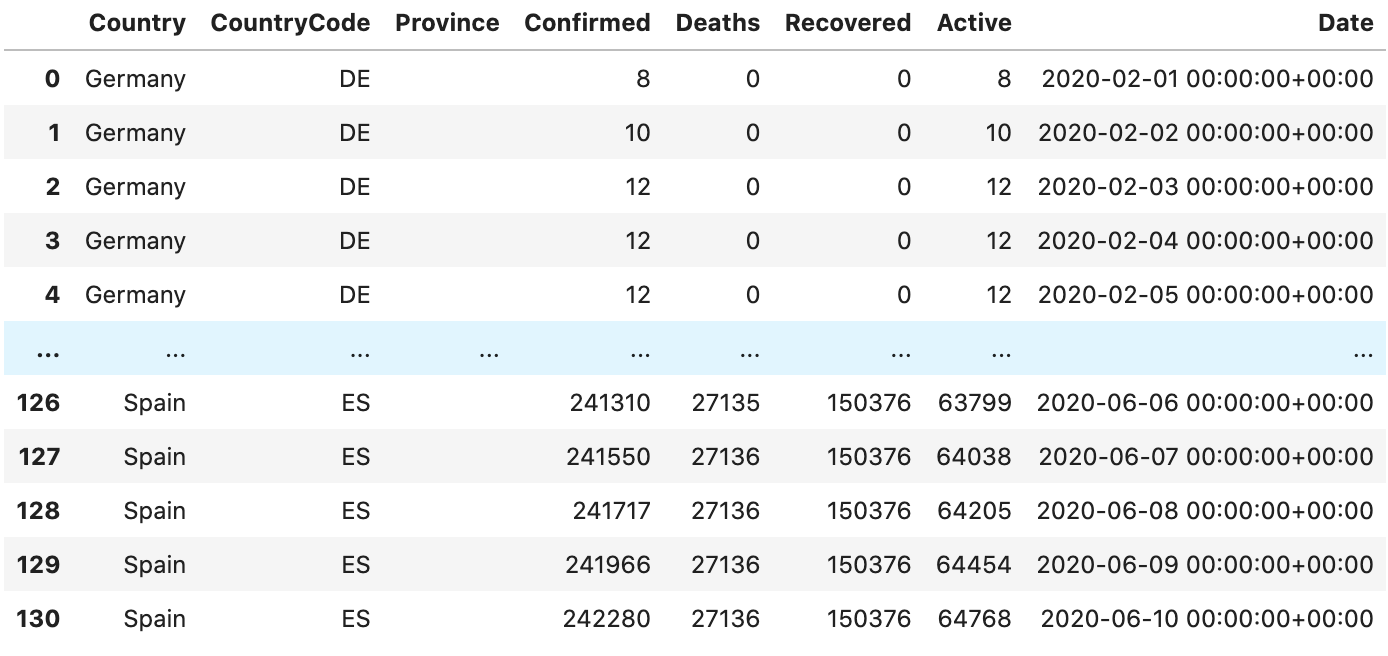
\includegraphics[width=\linewidth]{covid/countrys}
	\end{subfigure}
	\begin{subfigure}[b]{0.47\linewidth}
		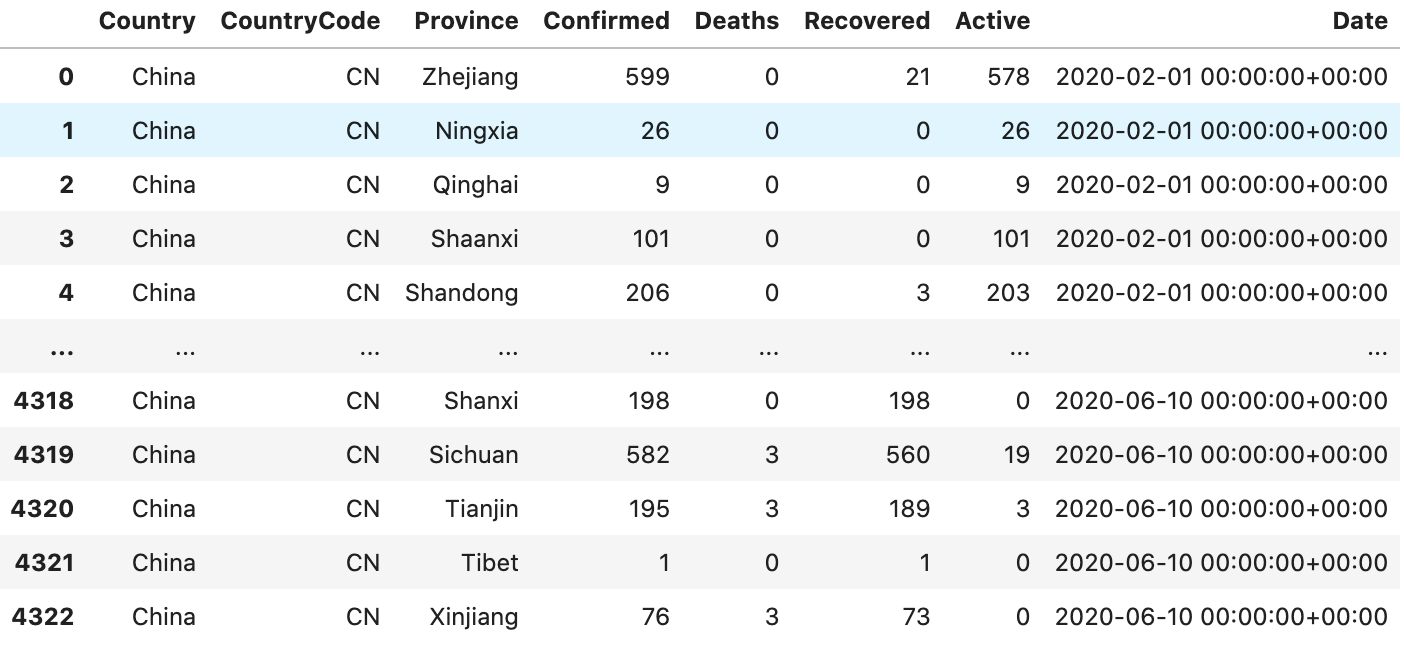
\includegraphics[width=\linewidth]{covid/provinces}
	\end{subfigure}
	\caption{Example of samples from the Johns Hopkins dataset.}
\end{figure}

\subsection{Processing data}

\begin{itemize}
	\item Importing data either online or offline.
	\item Choosing only country-level administrative regions.
	\item Selecting either most recent sample of each country or multiple samples over time for a single country.
	\item Visualizing either recent statistics of all countries or temporal data for a single country.
\end{itemize}
The world maps are drawn with Cartopy \cite{Cartopy}. Other figures are drawn with Matplotlib \cite{Hunter:2007}.

\begin{figure}[h]
	\centering
	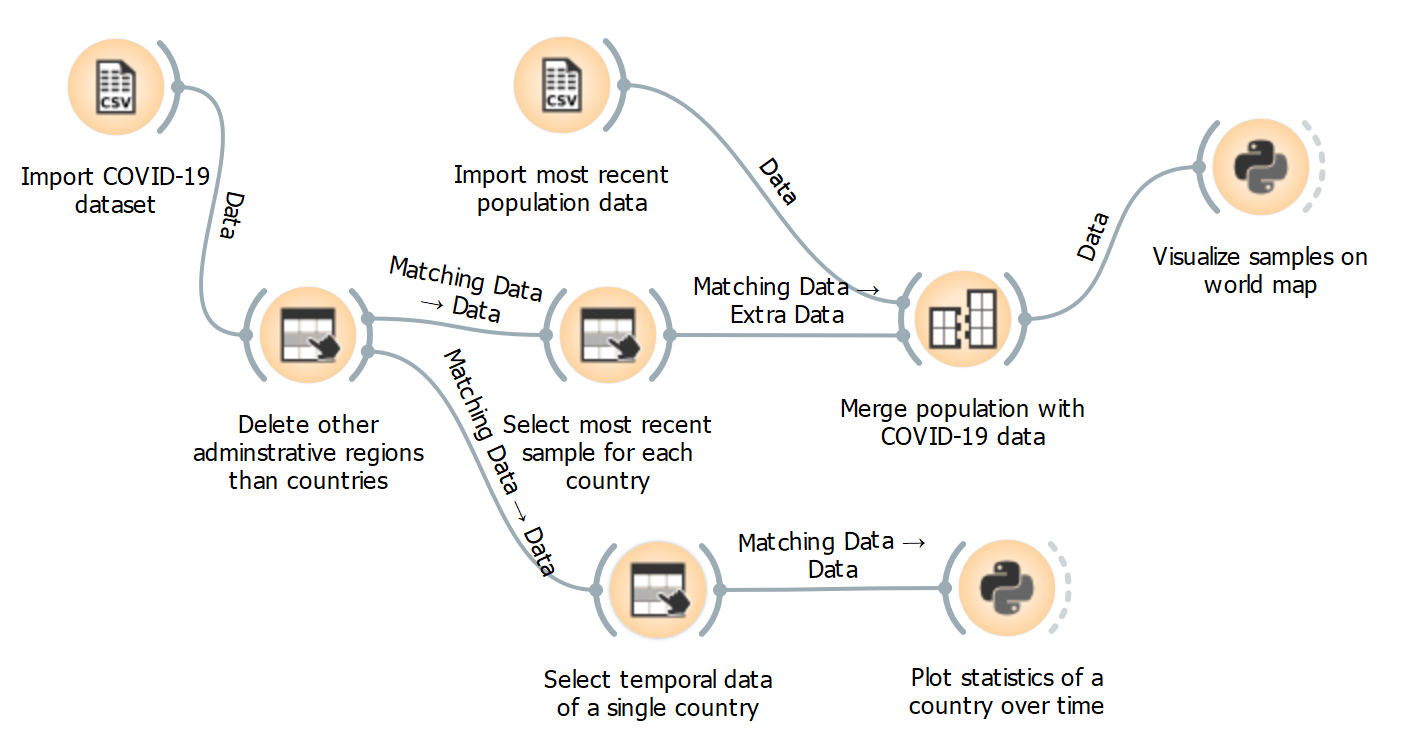
\includegraphics[width=0.80\linewidth]{covid/data_pipeline}
	\caption{Our general pipeline of processing Covid-19 datasets. Drawn using Orange \cite{Orange}}
\end{figure}


\subsection{Conclusion}
Having detailed Covid-19 data is a necessity for our research, since the effect of the pandemic on greenhouse gas emissions will be researched. In the end the datasets we have implemented are frequently updated, easy to access and use, consistent with each other, and have detailed information on cases. Therefore, we don't prefer one dataset over the other. Since we can access temporal data from individual countried throughout the pandemic, it will be easier to model the correlation between Covid-19 cases and greenhouse gas emissions.